% Final report. Numbers come from pretrained/results/tables/{main,ablations,sweep,retrieval,precision,stats}.md
% and results/final_stats.json, produced by scripts/make_tables.py, scripts/final_stats.py and scripts/make_figures.py.
%   cd pretrained && .venv/bin/python scripts/make_tables.py && .venv/bin/python scripts/final_stats.py \
%     && .venv/bin/python scripts/make_figures.py && cd ../Reports/Final && latexmk -pdf PreTrained_Final.tex
\documentclass[11pt,a4paper]{article}

\usepackage[margin=2.2cm]{geometry}
\usepackage[T1]{fontenc}
\usepackage{lmodern}
\usepackage{microtype}
\usepackage{amsmath}
\usepackage{xcolor}
\usepackage{booktabs}
\usepackage{tabularx}
\usepackage{array}
\usepackage{enumitem}
\usepackage{caption}
\usepackage{float}
\usepackage{graphicx}
\usepackage{titlesec}
\usepackage{tikz}
\usetikzlibrary{arrows.meta,positioning,fit,backgrounds,calc}
\usepackage[hidelinks]{hyperref}

\definecolor{accent}{HTML}{0E6B5C}
\definecolor{soft}{HTML}{E4F1EE}
\definecolor{warn}{HTML}{B4492C}
\definecolor{muted}{HTML}{56635E}

\titleformat{\section}{\large\bfseries\color{accent}}{\thesection}{0.6em}{}
\titleformat{\subsection}{\normalsize\bfseries}{\thesubsection}{0.5em}{}
\titlespacing*{\section}{0pt}{1.1em}{0.4em}
\titlespacing*{\subsection}{0pt}{0.8em}{0.3em}
\setlist{itemsep=1pt,topsep=3pt,leftmargin=1.4em}
\captionsetup{font=small,labelfont=bf}
\newcolumntype{L}{>{\raggedright\arraybackslash}X}
\newcolumntype{P}[1]{>{\raggedright\arraybackslash\hyphenpenalty=10000}p{#1}}
\renewcommand{\arraystretch}{1.15}
\setlength{\emergencystretch}{3em}

\newcommand{\up}[1]{\textbf{\color{accent}#1}}
\newcommand{\down}[1]{\textbf{\color{warn}#1}}
\let\oldpm\pm\renewcommand{\pm}{\ensuremath{\,\oldpm\,}}

\begin{document}

\begin{center}
  {\LARGE\bfseries Requirements as the Oracle}\\[3pt]
  {\large Generating REST API Tests from Vague Requirements Without Learning the Bugs They Should Catch}\\[6pt]
  {\large Final report}\\[8pt]
  {\large\bfseries Team PreTrained}\\[4pt]
  {\small\begin{tabular}{@{}l@{\hspace{1.2em}}l@{\hspace{3em}}l@{\hspace{1.2em}}l@{}}
Sohail Memon & 2025201075 & Mohd Ahmad & 2025201029\\
Kathan Patel & 2025201039 & Md Taufique Hussain & 2025202007
\end{tabular}}\\[6pt]
  {\small Code and results: \url{https://github.com/SohailTSM/Requirements-as-the-Oracle}}
\end{center}

\begin{abstract}\noindent
LLM-generated API tests are only useful if they encode the \emph{expected} behaviour. We study two problems on RESTestBench (3 services, 106 requirements, 228 planted bugs) with a single small open model, Llama~3.1~8B. First, requirements in practice are vague. Second, when a refinement loop repairs a test against a possibly buggy service, the test can learn the bug. Our agent retrieves the relevant operations, derives checks, writes a structured plan instead of code, cleans the plan against the specification, compiles it to pytest, runs it and refines it under a guard. On vague requirements it catches 12.7\% of planted bugs, against 2.6\% for single-step generation ($p<0.001$). Overall that is on par with RESTestBench's refinement loop (11.3\%, n.s.). When tests are refined against the buggy service, which is the realistic case, our agent keeps its score (14.8\%) while the refinement loop drops to 4.3\% ($+10.5$ points, 95\% CI $[5.6, 15.7]$, $p<0.001$). The refinement loop's adaptation gap is 7.0 points ($p=0.004$); ours is indistinguishable from zero for every variant. Ablations show that the deterministic executor ($-11.8$ points) and specification clean-up ($-7.5$) carry the gain. The derived checks, retrieval, judge and fine-tuning show no effect beyond run-to-run noise. Two humans labelled 181 items with $\kappa=0.84$. Against them, the Llama judge used for offline check scoring reaches only $\kappa=0.03$--$0.27$, so we report human-labelled precision numbers.
\end{abstract}

%-------------------------------------------------------------------- 1
\section{Introduction}
Crash-oriented REST testing tools (EvoMaster, RESTler, AutoRestTest~\cite{autoresttest}) use HTTP 5xx or schema violations as the oracle. A requirement violation that returns \texttt{200~OK}, such as a user deleting another user's data, is invisible to them. Catching such bugs needs the expected behaviour, which lives in natural-language requirements.

RESTestBench~\cite{restestbench} measured how well LLMs turn requirements into tests. Results are good with precise requirements but collapse with vague ones, the realistic case. A refinement loop (run, read the HTTP trace, regenerate) helps, but on a faulty service the model ``adapts its assertions to match the faulty behaviour'': the refined test encodes the bug as correct. The paper measures this effect but proposes no remedy. LLM-generated oracles are known to capture actual rather than expected behaviour~\cite{konstantinou}.

Our re-analysis of RESTestBench's released files (proposal, \S5.1) found that the refinement prompt's few-shot example teaches copying the observed value. Llama~3.1~8B's whole refinement gain on vague requirements (3.1\% $\to$ 12.3\%) disappears when it refines against the buggy service (3.5\%).

\textbf{Target user.} Backend and QA engineers who have user stories and an OpenAPI specification, and want tests that check behaviour, cheaply enough to run with a small local model.

%-------------------------------------------------------------------- 2
\section{Literature review}
\begin{itemize}
\item \textbf{Crash/schema fuzzers:} AutoRestTest~\cite{autoresttest}, LlamaRestTest~\cite{llamaresttest}, Schemathesis. Their oracle cannot see 200-returning logic bugs. We include Schemathesis as baseline E.
\item \textbf{Response-judging agents:} LogiAgent~\cite{logiagent}, ARMeta~\cite{armeta}. The judge sees the response before deciding, so it shares the bias we target. We include a LogiAgent-style judge as baseline B4.
\item \textbf{Oracle generation without requirements:} SATORI~\cite{satori}, MASTOR~\cite{mastor}. These derive truth from the specification or the implementation.
\item \textbf{Requirement-based generation:} APITestGenie~\cite{apitestgenie} and RESTestBench's own tools~\cite{restestbench}. We include the latter as B1/B2. None of these protects refinement from learning the bug.
\end{itemize}

%-------------------------------------------------------------------- 3
\section{Research questions and hypotheses}
\begin{description}[leftmargin=0pt,labelsep=0.4em]
\item[RQ1 (vague requirements).] Given only a vague requirement and the OpenAPI specification, can an 8B agent generate tests that catch requirement bugs, and how much of the vague-to-precise gap does it close?
\item[RQ2 (safe refinement).] Does restricted refinement remove bug adaptation without raising false alarms on the correct service?
\item[RQ3 (component value).] Which components contribute measurably, and which variant of each works best?
\end{description}
\textbf{H1:} deriving implied checks raises the score on vague requirements well above single-step generation. \textbf{H2:} with restricted refinement, the adaptation gap is $\approx0$ and false alarms are no higher than with unrestricted refinement. \textbf{H3:} tool-based execution sharply reduces tests that fail on the correct service.

%-------------------------------------------------------------------- 4
\section{Dataset}
\textbf{Benchmark used: RESTestBench}~\cite{restestbench}, released with its paper:
\begin{itemize}
\item FastAPI (Python), NestJS RealWorld (TypeScript) and TodoApp (.NET), run in Docker;
\item 63 / 29 / 14 requirements, each in a vague and a precise wording;
\item 141 / 65 / 22 hand-written planted bugs (mutants);
\item the unmodified scoring harness.
\end{itemize}
The agent sees only the requirement text and the specification. FastAPI was the development service; NestJS and TodoApp were held out from every design decision.

\textbf{Data we created.} RESTestBench has no labels below the test level, so we built the following (all in \texttt{pretrained/gold/} and \texttt{pretrained/finetune/} in the repository):
\begin{itemize}
\item \textbf{Gold operations} for all 106 requirements: the API operations each reference test calls, parsed from the benchmark's reference tests with the Python AST and matched to the specification. They are the ground truth for retrieval Recall@5 and MRR.
\item \textbf{Gold checks:} 268 atomic expected-behaviour checks (FastAPI 148, NestJS 94, TodoApp 26), drafted with an AI assistant by splitting the precise requirements, which are human-written. They are the ground truth for the precision layer and the SFT targets. Two humans validated a sample of them (\S\ref{sec:human}).
\item \textbf{Reference plans:} 10 JSON plans for FastAPI requirements, used to test the compiler and runtime.
\item \textbf{Human labels:} 181 items over 45 requirements (stratified, fixed seed), labelled independently by two team members (\S\ref{sec:human}).
\item \textbf{Fine-tuning data:} SFT examples (vague requirement $\to$ checks) in leave-one-service-out folds of 86 / 154 / 184 examples; DPO preference pairs from our own refinement histories, with the guarded plan preferred over the plan that copied or changed an expected value to the observed one (1{,}273 pairs from FastAPI runs; 143 from NestJS and TodoApp, which form the FastAPI-held-out fold, the only one trained).
\end{itemize}

%-------------------------------------------------------------------- 4
\section{Methodology}
\begin{figure}[H]\centering
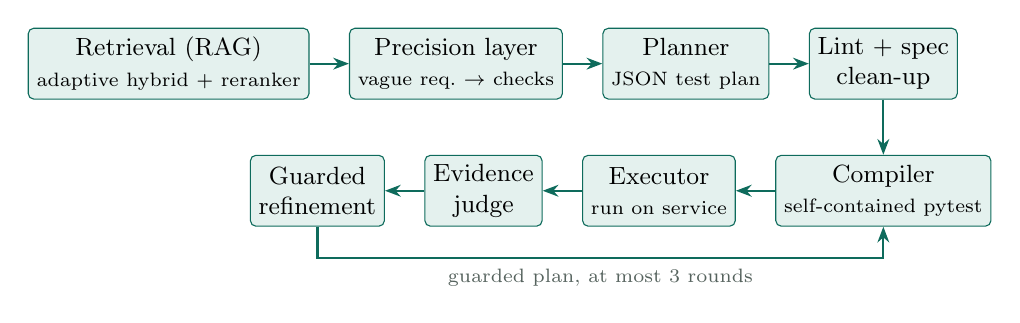
\begin{tikzpicture}[node distance=4mm and 5mm, box/.style={draw=accent, fill=soft, rounded corners=2pt, align=center, font=\small, minimum height=9mm, inner sep=3pt}, arr/.style={-{Stealth[length=2mm]}, accent, thick}]
\node[box] (ret) {Retrieval (RAG)\\\scriptsize adaptive hybrid + reranker};
\node[box, right=of ret] (pre) {Precision layer\\\scriptsize vague req.\ $\to$ checks};
\node[box, right=of pre] (plan) {Planner\\\scriptsize JSON test plan};
\node[box, right=of plan] (lint) {Lint + spec\\clean-up};
\node[box, below=7mm of lint] (comp) {Compiler\\\scriptsize self-contained pytest};
\node[box, left=of comp] (run) {Executor\\\scriptsize run on service};
\node[box, left=of run] (judge) {Evidence\\judge};
\node[box, left=of judge] (ref) {Guarded\\refinement};
\draw[arr] (ret) -- (pre); \draw[arr] (pre) -- (plan); \draw[arr] (plan) -- (lint); \draw[arr] (lint) -- (comp);
\draw[arr] (comp) -- (run); \draw[arr] (run) -- (judge); \draw[arr] (judge) -- (ref);
\draw[arr] (ref.south) -- ++(0,-4mm) -| node[pos=0.25, below, font=\scriptsize, muted]{guarded plan, at most 3 rounds} (comp.south);
\end{tikzpicture}
\caption{Final pipeline. Everything before the executor uses only the requirement and the specification frozen from the correct service.}
\end{figure}

\begin{enumerate}[label=(\arabic*)]
\item \textbf{Retrieval (RAG).} Each OpenAPI operation is one chunk (path, method, resolved schemas, description). BM25 and dense embeddings (bge-small) are fused. A cross-encoder (MiniLM) reranks only requirements of at most 30 words, since it hurts long precise ones (``adaptive''). Operations needed for authentication are added by dependency closure.
\item \textbf{Precision layer (reasoning).} The LLM expands the requirement into atomic checks, guided by a catalogue of implied properties: round-trip, echo, ownership, before/after deltas, filter soundness. In the final configuration, 5 sampled drafts are merged (self-consistency). Each check is tagged \emph{meaning} (locked) or \emph{format} (changeable only with specification evidence).
\item \textbf{Plan, not code (tool calling).} The LLM writes a JSON plan (actors, steps, checks). A linter checks it against the specification (unknown operations, references to fields that do not exist, impossible comparisons), and the LLM repairs flagged plans once.
\item \textbf{Specification clean-up.} Deterministic, specification-only fixes:
  \begin{itemize}
  \item drop checks that can never pass;
  \item generalise status codes the requirement does not state (\texttt{200}$\to$\texttt{2xx});
  \item replace invented credentials;
  \item redirect misdirected references;
  \item fill path parameters.
  \end{itemize}
\item \textbf{Compiler and executor (tools).} A compiler turns the plan into a self-contained pytest file. The runtime creates actors with valid credentials, logs in, passes IDs and joins every path to the service base URL.
\item \textbf{Guarded refinement and judge (agentic).} On a failure, the agent decides whether to refine, stop or relax a format check. The rules are:
  \begin{itemize}
  \item Assertion failures are reported without the observed value.
  \item A guard restores any change to a locked check, and blocks new expected values equal to a value the service just returned.
  \item Field repairs must name fields the specification documents.
  \item The judge may blame the test only with evidence from the requirement or the specification. An \textsc{API\_BUG} verdict ends the loop.
  \end{itemize}
\item \textbf{Fine-tuning.} QLoRA SFT of the precision layer (one model per held-out service) and DPO preferring ``report the bug'' over ``copy the observed value'' (Unsloth + TRL on Kaggle T4s, exported to 4-bit GGUF for Ollama).
\end{enumerate}
We also built and compared these alternatives in a component sweep: a single ReAct agent with tools; multi-persona and blackboard multi-agent designs; tools exposed over an MCP server; reviewer and debugger agents over A2A; and three amounts of content passed between agents (full trace, summary, verdict only).

%-------------------------------------------------------------------- 5
\section{Experiment runs}
\textbf{Model and compute.}
\begin{itemize}
\item Every LLM role, ours and the baselines', uses Llama~3.1~8B Instruct, 4-bit Q4\_K\_M, under Ollama: 24k context, temperature 0.2, at most 3 refinement rounds.
\item The models were served from free Kaggle T4 GPUs on the four team accounts, through Cloudflare tunnels.
\item A local dispatcher queued all requests and failed over between servers: 105{,}044 requests, 99.8\% answered, 251M tokens.
\item The services ran on a laptop, with up to 10 Docker copies at once.
\end{itemize}

\textbf{Baselines.}
\begin{enumerate}[label=\textbf{B\arabic*}]
\item RESTestBench single-step generation.
\item RESTestBench refinement loop, unchanged.
\item B2 with only the prompts fixed: copying example removed, generator warned, judge feedback passed on, \textsc{API\_BUG} outcome added.
\item LogiAgent-style response judge.
\end{enumerate}
\textbf{E}: the Schemathesis fuzzer, which uses no requirements.

\textbf{Metrics.}
\begin{itemize}
\item \emph{Caught}: RESTestBench's score, the \% of planted bugs killed by tests generated while interacting with the correct service. A test counts only if it passes on the correct service.
\item \emph{Mutant-gen}: the same score for tests generated while interacting with the buggy service, which is the realistic case.
\item \emph{Adaptation gap}: Caught $-$ Mutant-gen.
\item \emph{Fail-OK}: share of tests failing on the correct service (false alarms).
\item Per capability: retrieval Recall@5 and MRR; precision-layer check recall and contradiction rate (human-labelled); planner and lint failure rates; setup-error rate (tool calls); judge verdict accuracy; tampering attempts blocked and accepted; ReAct tool-call validity; cost per test.
\end{itemize}

\textbf{Protocol and statistics.}
\begin{itemize}
\item \textbf{Sweep:} one component varied at a time on FastAPI, vague wording, 1 run each.
\item \textbf{Finals:} the final configuration and 2 runner-ups; all services, both wordings, 3 runs each. Every baseline also ran 3 times.
\item \textbf{Ablations:} the final configuration minus one component, all services, vague wording, 1 run each.
\item \textbf{Statistics:}
  \begin{itemize}
  \item Unit: the requirement ($n=106$), its score averaged over runs.
  \item Paired Wilcoxon signed-rank tests, Holm-corrected within each family, with rank-biserial $r$.
  \item Bootstrap 95\% CIs of the pooled difference, resampling requirements.
  \end{itemize}
\item \textbf{Freeze:} every decision was logged with its reason, and the experiments were frozen on 11 Nov.
\end{itemize}

%-------------------------------------------------------------------- 6
\section{Evaluation}
\subsection{RQ1: vague requirements}
\begin{table}[H]\centering\small\setlength{\tabcolsep}{4.5pt}
\begin{tabular}{llrrrrrr}\toprule
Tool & Wording & FastAPI & NestJS & TodoApp & \textbf{All} & Mutant-gen & Fail-OK\\\midrule
B1 single-step & vague & 4.3\pm1.4 & 0.0\pm0.0 & 0.0\pm0.0 & 2.6\pm0.9 & -- & 97.2\\
B2 refinement & vague & \textbf{17.5}\pm2.3 & 0.0\pm0.0 & 4.5\pm0.0 & 11.3\pm1.4 & 4.3\pm2.0 & 85.2\\
B3 prompt-fixed & vague & 4.5\pm2.9 & 0.0\pm0.0 & 0.0\pm0.0 & 2.8\pm1.8 & 3.1\pm0.9 & 96.9\\
B4 response judge & vague & 6.6\pm0.4 & 3.1\pm4.1 & 18.2\pm0.0 & 6.7\pm1.1 & -- & \textbf{40.6}\\
E fuzzer & -- & 13.9\pm7.8 & 0.0\pm0.0 & 9.1\pm0.0 & 9.5\pm4.8 & -- & 70.8\\
\textbf{Ours (final)} & vague & 12.5\pm3.2 & 2.6\pm3.2 & \textbf{43.9}\pm6.9 & \textbf{12.7}\pm2.7 & \textbf{14.8}\pm1.2 & 70.4\\\midrule
B1 single-step & precise & 39.7\pm2.6 & 5.1\pm1.8 & 1.5\pm2.6 & 26.2\pm1.8 & -- & 77.4\\
B2 refinement & precise & \textbf{47.8}\pm2.2 & 6.2\pm2.7 & 0.0\pm0.0 & \textbf{31.3}\pm0.7 & \textbf{24.8}\pm0.6 & 68.6\\
B3 prompt-fixed & precise & 37.6\pm2.5 & 5.6\pm4.9 & 0.0\pm0.0 & 24.9\pm0.3 & 25.4\pm3.0 & 78.0\\
B4 response judge & precise & 13.5\pm2.5 & 10.3\pm5.8 & 4.5\pm0.0 & 11.7\pm2.9 & -- & \textbf{56.0}\\
\textbf{Ours (final)} & precise & 20.6\pm5.1 & \textbf{22.1}\pm3.9 & 1.5\pm2.6 & 19.2\pm2.2 & 16.0\pm3.0 & 77.7\\
\bottomrule\end{tabular}
\caption{Planted bugs caught (\%), mean $\pm$ sd over 3 runs, Llama~3.1~8B for every tool. ``--'': the tool does not refine against the service, so no mutant-gen score exists.}
\label{tab:main}
\end{table}

\begin{table}[H]\centering\small
\begin{tabular}{lrrrrr}\toprule
Ours (final) vs & $\Delta$ caught & 95\% CI & better / worse req. & $p$ (Holm) & $r$\\\midrule
\multicolumn{6}{l}{\emph{Vague: caught}}\\
B1 single-step & $+10.1$ & $[+5.2, +15.2]$ & 35 / 4 & $<$0.001 & $+0.75$\\
B2 refinement & $+1.5$ & $[-5.3, +7.9]$ & 30 / 22 & 1.000 & $+0.09$\\
B3 prompt-fixed & $+9.9$ & $[+5.5, +14.6]$ & 33 / 5 & $<$0.001 & $+0.85$\\
B4 response judge & $+6.0$ & $[+1.0, +11.1]$ & 32 / 11 & 0.032 & $+0.45$\\
E fuzzer & $+3.2$ & $[-2.5, +9.1]$ & 26 / 19 & 1.000 & $+0.20$\\
\multicolumn{6}{l}{\emph{Vague: mutant-gen (refined against the buggy service)}}\\
B2 refinement & $\mathbf{+10.5}$ & $[+5.6, +15.7]$ & 42 / 10 & $<$0.001 & $+0.69$\\
B3 prompt-fixed & $+11.7$ & $[+6.8, +16.8]$ & 45 / 5 & $<$0.001 & $+0.80$\\
\multicolumn{6}{l}{\emph{Precise: caught}}\\
B1 single-step & $-7.0$ & $[-15.9, +2.2]$ & 26 / 28 & 1.000 & $-0.19$\\
B2 refinement & $-12.1$ & $[-20.8, -3.5]$ & 20 / 37 & 0.062 & $-0.49$\\
B4 response judge & $+7.5$ & $[+2.0, +12.8]$ & 30 / 14 & 0.251 & $+0.27$\\
\multicolumn{6}{l}{\emph{Precise: mutant-gen}}\\
B2 refinement & $-8.8$ & $[-16.6, -0.9]$ & 32 / 35 & 1.000 & $-0.16$\\
\bottomrule\end{tabular}
\caption{Paired comparisons per requirement ($n=106$). $\Delta$ = pooled percentage points, ours minus other. Wilcoxon $p$ values are Holm-corrected within each block of comparisons (the full set, including runner-ups, is in \texttt{results/tables/stats.md}).}
\label{tab:stats}
\end{table}

\textbf{Reading.}
\begin{itemize}
\item \textbf{The pipeline lifts vague requirements well above single-step generation.} It scores $+10.1$ points over B1 and $+9.9$ over B3, both $p<0.001$ with large effects. This closes 35\% of the way from B1-vague (2.6) to the best precise score (B2, 31.3).
\item \textbf{Against B2 it is a draw on the correct service.} The difference is $+1.5$, CI $[-5.3,+7.9]$.
\item \textbf{The win comes in the realistic setting.} With refinement against the buggy service, ours keeps 14.8\% while B2 falls to 4.3\%. That is $+10.5$ points, $3.4\times$, $p<0.001$.
\item \textbf{The held-out services behave differently from FastAPI.} B2 is strongest on FastAPI. Ours wins on the held-out services: TodoApp vague 43.9 vs at most 18.2; NestJS precise 22.1 vs at most 10.3. On TodoApp the baselines register users with weak passwords that an undocumented password policy rejects. Our runtime creates valid actors.
\item \textbf{Weakness: precise wording.} B2 beats ours by 12.1 points (CI excludes 0; Holm $p=0.062$). Our precision layer and clean-up generalise status codes and drop specific checks, which wastes the extra information a precise requirement gives. Our score barely rises from vague to precise (12.7 $\to$ 19.2), while B2's nearly triples.
\end{itemize}

\subsection{RQ2: bug adaptation and safe refinement}
\begin{figure}[H]\centering
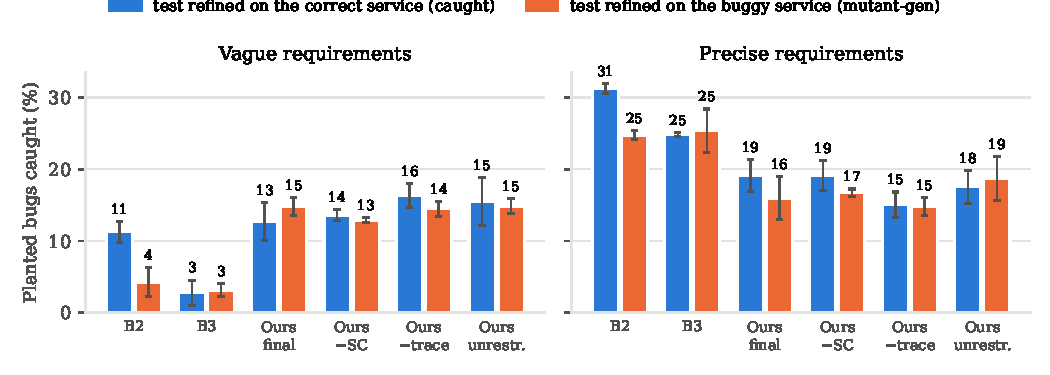
\includegraphics[width=\linewidth]{figures/adaptation.pdf}
\caption{Score of tests refined on the correct service (blue) vs on the buggy service (orange), mean $\pm$ sd over 3 runs. B2's tests lose most of their value when they are refined against the buggy service; ours do not. SC = self-consistency.}
\label{fig:adapt}
\end{figure}
\begin{table}[H]\centering\small
\setlength{\tabcolsep}{4pt}\begin{tabular}{llrrrr}\toprule
Tool & Wording & Gap & $p$ & Rounds copying a value & Copies in next plan\\\midrule
B2 refinement & vague & \down{7.0\pm2.8} & 0.004 & 261 / 1931 (13.5\%) & all\\
B2 refinement & precise & \down{6.5\pm1.3} & 0.004 & 151 / 1825 (8.3\%) & all\\
B3 prompt-fixed & vague & $-0.3$\pm1.3 & 0.86 & 2 / 33 (6.1\%) & all\\
Ours (final) & vague & $-2.1$\pm3.4 & 0.058 & 21 / 739 tried (2.8\%) & 3 / 787 (0.4\%)\\
Ours (final) & precise & 3.2\pm3.0 & 0.30 & 57 / 960 tried (5.9\%) & 8 / 972 (0.8\%)\\
Ours, unrestricted & vague & 0.6\pm3.8 & 0.68 & -- & 33 / 807 (4.1\%)\\
Ours, unrestricted & precise & $-1.1$\pm2.1 & 0.20 & -- & 135 / 932 (14.5\%)\\
\bottomrule\end{tabular}
\caption{Adaptation gap (caught $-$ mutant-gen, mean $\pm$ sd over runs) with a per-requirement Wilcoxon test, and value copying in refinement. For ours, ``copies reaching the test'' compares each next executed plan with the values the service returned. The few residual cases in the final configuration are permitted format changes backed by specification evidence, or values that coincide with the correct behaviour.}
\label{tab:adapt}
\end{table}
\begin{itemize}
\item \textbf{B2 learns the bugs.} Its gap is 7.0 points on vague and 6.5 on precise wording (both $p=0.004$). In 8--14\% of its refinement rounds it adds an asserted literal taken from the previous response. B3, whose judge almost always answers \textsc{API\_BUG}, barely refines (33--74 rounds) and so neither gains nor adapts.
\item \textbf{Our agent does not, in any variant.} No gap differs from zero, and all mutant-gen differences between our variants are within noise ($|\Delta|\le2.7$, all $p>0.15$).
\item \textbf{The guard works as a mechanism.} It blocked 512 (vague) and 773 (precise) tampering attempts, mostly attempts to change a locked check (1{,}196 restored across both wordings). It cut copied values reaching the test from 4.1--14.5\% (unrestricted) to under 1\%.
\item \textbf{But the guard is not what removes adaptation here.} The unrestricted variant copies values yet shows no gap and the same mutant-gen ($-0.1$, n.s.). Its false-alarm rate is also no different (Fail-OK 68.2 vs 70.4).
\item \textbf{Where the protection comes from.} It comes mainly from the structure:
  \begin{itemize}
  \item checks are derived before any execution, so the requirement, not the response, defines them;
  \item most refinement rounds repair setup, not expectations (58--70\% of rounds have a setup error, \S\ref{sec:steps});
  \item a copied value in our plans usually equals correct behaviour that a planted bug does not touch.
  \end{itemize}
\end{itemize}
So H2 is supported for the pipeline, not for the guard alone. The restriction is cheap insurance that removes visible tampering; on this benchmark it shows no measurable effect on scores.

\subsection{Intermediate steps, per capability}\label{sec:steps}
\begin{table}[H]\centering\small
\begin{tabularx}{\linewidth}{@{}P{2.6cm}LP{5.0cm}@{}}\toprule
Capability / step & Metric & Final configuration\\\midrule
RAG: retrieval & Recall@5 / all needed in top 5 / MRR (106 req.) & vague 0.89 / 0.81 / 0.87; precise 0.90 / 0.80 / 0.78 (BM25 vague: 0.79 / 0.69 / 0.70)\\
Reasoning: precision layer & Gold checks fully covered / soft recall; derived checks contradicting the gold (human labels, 20 req.) & 0.29--0.41 / 0.54--0.58; contradiction 0.09 (Llama judge on the same items: 0.30)\\
Reasoning: planner & Plans that fail to parse after retry; plans with lint issues & 2.9\% / 51\% (vague); 3.1\% / 63\% (precise)\\
Tool calling: executor & Rounds with a setup error (missing field reference / setup call rejected) & 58\% vague (662 / 363), 70\% precise (425 / 891)\\
Agentic: judge & \textsc{API\_BUG} verdicts on the correct service, where every failure is the test's fault & 117 of 117 (vague), 95 of 96 (precise): no discrimination\\
Safety: refinement & Tampering attempts blocked / accepted & 512 / 0 (vague), 773 / 0 (precise)\\
Safety: actions & Calls outside the service; forbidden test edits (skip, removed asserts) & 0 possible: the runtime joins every path to the base URL (2 plan steps naming another host became invalid requests); 0 (tests are compiled)\\
Cost & LLM calls / tokens / seconds per generated test & 7.7 / 13.9k / 123 s (vague); 8.0 / 16.5k / 183 s (precise)\\
\bottomrule\end{tabularx}
\caption{Step-level metrics from the agent histories of the final configuration (3 runs, 1{,}002 generated tests per wording).}
\end{table}
\textbf{The judge.} It answered \textsc{API\_BUG} for every failure on the correct service (212 of 213), and returned \textsc{TEST\_BUG} only 2 times in 826 verdicts. The 8B judge does not discriminate; it works as a stop rule. This matches the baselines: B3's judge answered \textsc{API\_BUG} in 36 of 36 TodoApp rounds. An evidence-restricted judge needs a stronger model than 8B.

\subsection{Human validation of the LLM judge}\label{sec:human}
Sohail and Kathan independently labelled 181 items (45 requirements, stratified sample):
\begin{itemize}
\item 63 judgements of whether a gold check is correct;
\item 118 coverage labels comparing the precision layer's checks with the gold checks.
\end{itemize}
\begin{itemize}
\item \textbf{Human--human agreement is high:} Cohen's $\kappa=0.84$ over 181 paired labels. The task is well defined.
\item \textbf{The gold data holds up:} 125 of 126 gold-check judgements were ``correct'' (0.8\% wrong).
\item \textbf{The Llama judge does not agree with humans:} $\kappa=0.03$ on gold coverage and $0.27$ on derived checks. It calls three times as many contradictions (20 vs 6 of 67), calls ``partial'' coverage ``full'' (25 of the 102 coverage labels), and answers from the wrong label set in 9 of 118 cases.
\end{itemize}
Consequence: the offline precision-layer table scored by Llama (Table~\ref{tab:prec}) is unreliable in absolute terms. Only the human-labelled rates are claims. The main results do not use this judge: mutation scores come from the harness.
\begin{table}[H]\centering\small
\begin{tabular}{llrrr}\toprule
Precision layer (prompt v2) & Wording & Recall & Contradiction & Checks / req.\\\midrule
catalogue & vague & 0.39 & 0.27 & 3.6\\
direct rewrite & vague & 0.40 & 0.21 & 5.7\\
self-consistency & vague & 0.37 & 0.26 & 3.1\\
catalogue & precise & 0.47 & 0.14 & 6.8\\
\midrule
catalogue, \textbf{human labels} & vague & 0.29--0.41 (soft 0.54--0.58) & \textbf{0.09} & --\\
\bottomrule\end{tabular}
\caption{Offline precision layer against the gold checks (106 requirements), scored by the Llama judge, with the human-labelled sample below.}
\label{tab:prec}
\end{table}

\subsection{Failure analysis}
\begin{table}[H]\centering\small
\begin{tabular}{lrr}\toprule
Outcome of the test generated on the correct service (3 runs $\times$ 106) & Vague & Precise\\\midrule
Passes and catches at least one planted bug & 63 (20\%) & 61 (19\%)\\
Passes but catches no planted bug (checks too weak) & 31 (10\%) & 10 (3\%)\\
Fails: setup error (wrong field reference, rejected setup call) & 85 (27\%) & 136 (43\%)\\
Fails: a check contradicts the real behaviour; judge blamed the API & 112 (35\%) & 93 (29\%)\\
Fails: a check contradicts the real behaviour; rounds exhausted & 12 (4\%) & 3 (1\%)\\
No valid plan (planner failed) & 15 (5\%) & 15 (5\%)\\
\bottomrule\end{tabular}
\caption{Failure taxonomy, computed from the agent histories and the harness results.}
\end{table}
The two dominant failures are wrong checks (39\% vague) and setup errors (27\% vague, 43\% precise). Precise requirements name exact payloads, which likely leads the planner into more setup calls the service rejects. Across both wordings, the most frequent setup errors are FastAPI calls that need admin rights (403) and references to request fields that do not exist.

\textbf{Qualitative examples.}
\begin{itemize}
\item \textbf{Self-contradicting checks} (FastAPI, ``Verify that a second user cannot delete an item created by another user''). Self-consistency merged the check ``deleting another user's item is rejected (4xx)'' with a draft's ``\ldots{} still returns 200''. The test can never pass, and the judge blamed the API. A consistency check over derived checks would remove this class.
\item \textbf{The specification as a misleading oracle} (FastAPI, ``Check that log in rejects a wrong password''). The derived check ``rejection status is 422, the code documented for this operation'' follows the OpenAPI file, but the service returns 400. Specification evidence is not ground truth when the specification is incomplete.
\item \textbf{The guard at work} (FastAPI mutant, ``Delete a non-existing item and confirm the API reports `Item not found'\,''). Refinement tried to add a status check equal to the status the buggy service had just returned. The guard blocked it as a copied value, and the locked check kept the test able to kill the mutant.
\item \textbf{Weak passwords} (TodoApp, all LLM baselines). Generated tests register users with passwords like \texttt{password123}, which the service's undocumented policy rejects, so almost every baseline test fails setup. Our runtime generates valid credentials, which explains most of our TodoApp margin.
\end{itemize}

%-------------------------------------------------------------------- 7
\section{Ablations (RQ3: which components matter)}
\begin{figure}[H]\centering
\begin{minipage}[c]{0.5\linewidth}\centering
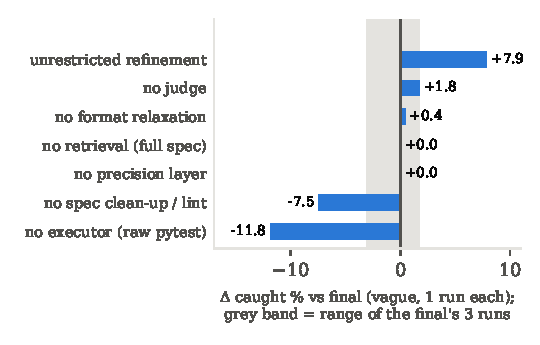
\includegraphics[width=\linewidth]{figures/ablations.pdf}
\end{minipage}\hfill
\begin{minipage}[c]{0.47\linewidth}\small
\begin{tabular}{lrr}\toprule
Removed (vague, 1 run) & All & Fail-OK\\\midrule
final (3 runs) & 12.7 & 70.4\\
executor (raw pytest) & 0.9 & 98.1\\
spec clean-up / lint & 5.3 & 85.8\\
precision layer & 12.7 & 75.5\\
retrieval (full spec) & 12.7 & 71.7\\
format relaxation & 13.2 & 74.5\\
judge & 14.5 & 65.1\\
restricted refinement & 20.6 & 60.4\\
\bottomrule\end{tabular}
\end{minipage}
\caption{Ablations: the final configuration minus one component, all services, vague. The grey band is the range of the final's own 3 runs (9.6--14.5). ``Restricted refinement'' was re-run 3 times: 15.5\pm3.3, $\Delta=+2.8$, $p=0.27$, so its single +7.9 did not replicate.}
\label{fig:abl}
\end{figure}
\begin{itemize}
\item \textbf{Clear effects: the executor and specification clean-up (support H3).}
  \begin{itemize}
  \item Without the plan-and-compile executor, 98\% of tests fail on the correct service and the score falls to 0.9\%. The model writes placeholders such as \texttt{Bearer YOUR\_TOKEN}.
  \item Without clean-up and lint the score falls to 5.3\%. The clean-up fires constantly: per 1{,}002 generated tests (vague) it dropped 443 impossible checks, replaced 253 invented credentials, generalised 252 unstated status codes and redirected 143 references.
  \end{itemize}
\item \textbf{No measurable effect:} the precision layer, retrieval and format relaxation each leave the score at 12.7--13.2. Removing the judge raises caught slightly (14.5) but lowers mutant-gen (14.8 $\to$ 10.4), consistent with the judge acting as an early stop on buggy services. These are single runs inside the noise band.
\item \textbf{Combining the sweep's winners did not add up.} The final adds two sweep winners (full-trace content $+6.4$, self-consistency $+5.0$, single runs) to the default. In the finals, removing either one does not lower the score: the two runner-ups score 0.9 and 3.7 points \emph{higher} than the final, both n.s. The final configuration's own runs spread from 9.6 to 14.5, so single-run differences under about $\pm6$ points are not readable. We report this as a methodological lesson: the sweep's single runs over-selected noise.
\item \textbf{Fine-tuning shows no effect beyond noise.} SFT of the precision layer took 23--47 minutes per fold on a T4 (86/154/184 examples, final loss 0.19--0.35). DPO on the FastAPI-held-out fold had 143 pairs, loss $0.69\to0.14$, and took 133 minutes including export. On FastAPI (single sweep runs) the fine-tuned precision layer scored 17.0, SFT as the whole model 15.6 and SFT+DPO 14.2, against the default's 11.3--13.5. All are inside the noise, so the two larger DPO folds were not trained.
\item \textbf{Architecture.} A single ReAct agent with tools scored 5.0 and a blackboard design 3.5, against 12.0 for the fixed pipeline. Over 2{,}069 ReAct turns:
  \begin{itemize}
  \item 66\% were well-formed tool calls;
  \item 12\% wrote the call as plain text (we unwrap and execute these);
  \item 22\% called no tool at all;
  \item 25\% of generations ended in the fallback planner.
  \end{itemize}
  The 8B model is not a reliable controller, which is why the final design keeps control in code. MCP (12.1) and A2A (14.9) transport was neutral.
\item \textbf{4-bit vs fp16.} One fp16 run scored 13.6 against 12.7\pm2.7 for 4-bit ($\Delta=-0.9$, $p=0.54$; mutant-gen 14.3 vs 14.8). We found no measurable quantisation penalty, so reporting on 4-bit is justified.
\end{itemize}

%-------------------------------------------------------------------- 7
\section{Discussion: hypotheses}
\begin{itemize}
\item \textbf{H1: partly supported.} The full pipeline beats single-step generation clearly on vague requirements (+10.1, $p<0.001$). However, the precision layer itself does not account for it: removing it leaves the score unchanged, and human labels show it recovers only 29--41\% of gold checks fully. The gain comes from executable structure, not from deriving implied properties.
\item \textbf{H2: supported for the pipeline, not attributable to the guard.} The adaptation gap is $\approx0$ for every variant of ours, and 7.0 points for B2. False alarms do not rise with restriction. But unrestricted refinement shows the same result, so the plan structure, not the guard, is what protects the tests.
\item \textbf{H3: supported.} Tool-based execution moves Fail-OK from 98.1\% to 70.4\% and is the largest single effect ($-11.8$). Yet 70\% of tests still fail on the correct service, so execution reduces false alarms but does not solve them.
\end{itemize}

%-------------------------------------------------------------------- 8
\section{Limitations and threats to validity}
\begin{itemize}
\item \textbf{Scale.} One benchmark of 3 services. The proposal's optional extension (EMB/RESTgym services) was not done. With 106 requirements and 3 runs, differences below about 5 points are not detectable.
\item \textbf{Noise.} The final configuration's own runs range from 9.6 to 14.5. Sweep and ablation rows are single runs, and only effects larger than about $\pm6$ points are interpretable. The choice of the final configuration from single runs was not confirmed by the finals.
\item \textbf{Development service.} All design decisions were made on FastAPI. The held-out services favour us, but the clean-up rules (e.g.\ credential replacement) encode lessons learned while building on FastAPI.
\item \textbf{One model.} Every result is for Llama~3.1~8B 4-bit. The planned GPT-5 Nano reference was dropped to keep the study to one open model. Conclusions about the judge and the ReAct agent may not hold for larger models.
\item \textbf{Fine-tuning.} Fine-tuning was tested only in single sweep runs on FastAPI, with one DPO fold.
\item \textbf{The LLM judge.} The judge used for offline check scoring was shown to be unreliable; only its human-validated sample supports claims.
\end{itemize}

%-------------------------------------------------------------------- 9
\section{Conclusion and future work}
With a single 8B model, structure beats cleverness. A plan-compile-execute pipeline with specification clean-up lifts vague-requirement testing from 2.6\% to 12.7\%. It also stays robust when refined against a buggy service, where RESTestBench's refinement loop loses two-thirds of its score (14.8\% vs 4.3\%). The components that ask the 8B model to reason more did not measurably help: derived checks, an evidence judge, a ReAct controller and fine-tuning. Its judgements, both as the evidence judge and as the offline scorer, did not survive validation.

Future work:
\begin{itemize}
\item a consistency check over derived checks;
\item a stronger, validated judge;
\item using precise requirements without generalising their details away;
\item replicating on more services with more runs per configuration.
\end{itemize}

\section*{Acknowledgment}
We thank our course instructor, Prof.~Vasudeva Varma, and the TAs for their guidance, the RESTestBench authors for releasing their benchmark, and Kaggle for free GPU time.

\appendix
\section{Deviations from the proposal}
\begin{itemize}
\item \textbf{4-bit instead of fp16 for the reported runs:} one fp16 run confirms no measurable difference.
\item \textbf{No GPT-5 Nano reference:} single-model study (Llama only).
\item \textbf{DPO trained on one fold only:} the larger folds were dropped because the first showed no gain.
\item \textbf{The ablation ``minus fine-tuning'' is replaced by the sweep's fine-tuned rows:} the final configuration uses the base model.
\item \textbf{The planned paired Wilcoxon tests use the requirement as the unit.}
\end{itemize}

\section{Reproducibility}
\begin{itemize}
\item \textbf{Repository:} \url{https://github.com/SohailTSM/Requirements-as-the-Oracle}. Its \texttt{README.md} gives the setup, the commands to run one job or a whole queue, and the commands that rebuild every table and figure.
\item \textbf{Code:} the agent (\texttt{pretrained/agent/}), baselines (\texttt{tools\_ext/}), the queue runner and dispatcher (\texttt{scripts/}), fine-tuning jobs (\texttt{finetune/}) and server notebooks (\texttt{kaggle\_llm\_server/}) are in the repository.
\item \textbf{Configurations:} every configuration is a YAML file in \texttt{configs/agent/}.
\item \textbf{Results:} every reported number is regenerated from the result files by \texttt{make\_tables.py}, \texttt{final\_stats.py} and \texttt{make\_figures.py}.
\item \textbf{Decisions:} every design decision and its reason is recorded in \texttt{Plan/Decision\_Log.md}.
\end{itemize}

\begin{thebibliography}{99}\small
\setlength{\itemsep}{1pt}
\bibitem{restestbench} L.~Kogler, S.~Hangler, M.~Ehrhart, B.~Dornauer, R.~Wuersching, P.~Schrammel. \emph{RESTestBench: A Benchmark for Evaluating the Effectiveness of LLM-Generated REST API Test Cases from NL Requirements.} EASE 2026. arXiv:2604.25862.
\bibitem{autoresttest} M.~Kim et al. \emph{A Multi-Agent Approach for REST API Testing with Semantic Graphs and LLM-Driven Inputs (AutoRestTest).} ICSE 2025. arXiv:2411.07098.
\bibitem{llamaresttest} M.~Kim et al. \emph{LlamaRestTest: Effective REST API Testing with Small Language Models.} FSE 2025. arXiv:2501.08598.
\bibitem{logiagent} \emph{LogiAgent: Automated Logical Testing for REST Systems with LLM-Based Multi-Agents.} arXiv:2503.15079, 2025.
\bibitem{armeta} \emph{Multi-Agent LLM-based Metamorphic Testing for REST APIs (ARMeta).} arXiv:2605.28321, 2026.
\bibitem{satori} J.~C.~Alonso et al. \emph{SATORI: Static Test Oracle Generation for REST APIs.} ASE 2025. arXiv:2508.16318.
\bibitem{mastor} \emph{MASTOR: A Multi-Agent Approach to Semantic Test Oracle Generation for RESTful APIs.} arXiv:2606.10465, 2026.
\bibitem{apitestgenie} \emph{APITestGenie: Generating Web API Tests from Requirements and API Specifications with LLMs.} arXiv:2604.02039, 2026.
\bibitem{konstantinou} M.~Konstantinou et al. \emph{Do LLMs Generate Test Oracles that Capture the Actual or the Expected Program Behaviour?} arXiv:2410.21136, 2024.
\end{thebibliography}
\end{document}
